% Created 2012-07-06 Fr 10:18
\documentclass[11pt]{article}
\usepackage[utf8]{inputenc}
\usepackage[T1]{fontenc}
\usepackage{fixltx2e}
\usepackage{graphicx}
\usepackage{longtable}
\usepackage{float}
\usepackage{wrapfig}
\usepackage{soul}
\usepackage{textcomp}
\usepackage{marvosym}
\usepackage{wasysym}
\usepackage{latexsym}
\usepackage{amssymb}
\usepackage{hyperref}
\tolerance=1000
\usepackage{color}
\usepackage{listings}
\providecommand{\alert}[1]{\textbf{#1}}

\title{Example}
\author{Bernd Weiss}
\date{2012-07-06}
\hypersetup{
  pdfkeywords={},
  pdfsubject={},
  pdfcreator={Emacs Org-mode version 7.8.11}}

\begin{document}

\maketitle

\setcounter{tocdepth}{3}
\tableofcontents
\vspace*{1cm}


\definecolor{dkgreen}{rgb}{0,0.5,0}
\definecolor{dkred}{rgb}{0.5,0,0}
\definecolor{gray}{rgb}{0.5,0.5,0.5}

\lstset{basicstyle=\ttfamily\bfseries\footnotesize,
morekeywords={virtualinvoke},
%%keywordstyle=\color{blue},
%%ndkeywordstyle=\color{red},
commentstyle=\color{dkred},
%%stringstyle=\color{dkgreen},
numbers=left,
numberstyle=\ttfamily\tiny\color{gray},
stepnumber=1,
numbersep=10pt,
backgroundcolor=\color{white},
tabsize=4,
showspaces=false,
showstringspaces=false,
xleftmargin=.23in
}


\begin{abstract}
abstract abstract abstract abstract abstract abstract abstract abstract abstract 
\end{abstract}


\section{Introduction and some R code}
\label{sec-1}


Let's start with an equation: 

\begin{equation}
v^{*}_{j} = v_{j} + \tau^{2} 
\end{equation}

Now, some R code:


\lstset{language=R}
\begin{lstlisting}
## Create 100 normally distributed numbers 
x <- rnorm(100)
## Estimate mean
mean(x)
\end{lstlisting}

\begin{verbatim}
 [1] 0.1008427
\end{verbatim}

The mean of x is 0.101
\section{Plot a histogram}
\label{sec-2}




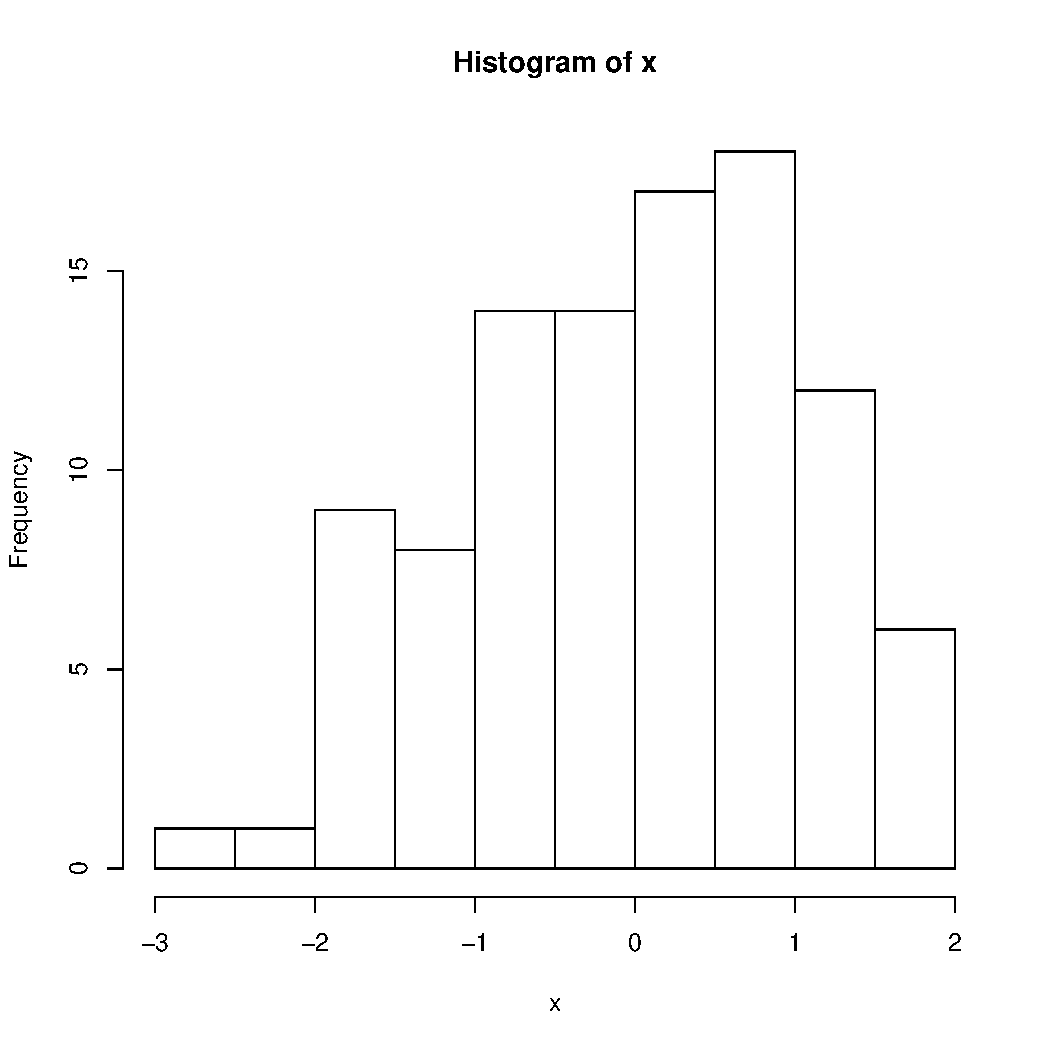
\includegraphics[width=.9\linewidth]{../fig/f_pub_histogram.pdf}





\begin{figure}[htb]
\centering
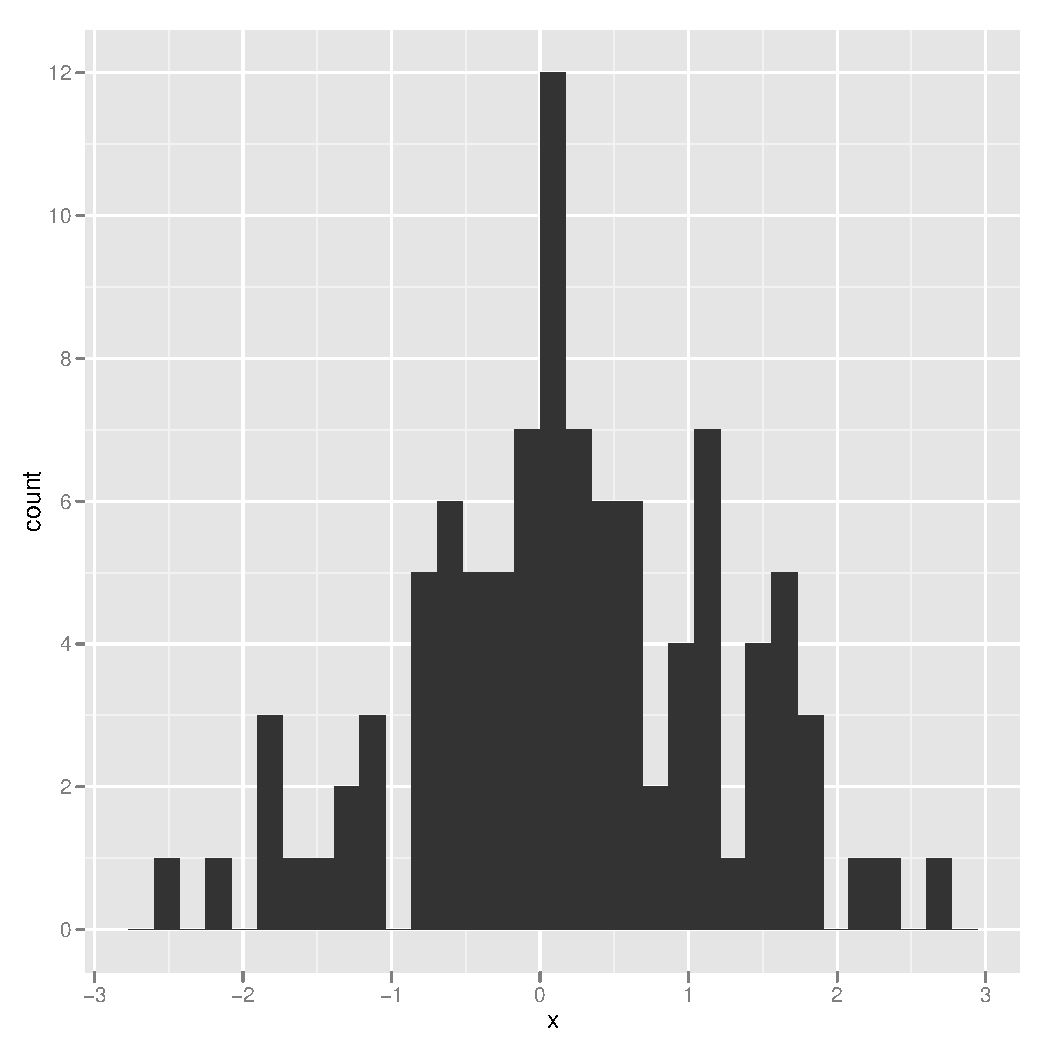
\includegraphics[width = 0.2\linewidth, clip]{../fig/f_pub_histogram_gg.pdf}
\caption{\label{f:ggplot}A beautiful ggplot2 plot}
\end{figure}

See Figure \ref{f:ggplot} blablabla
\section{Use the Bash!}
\label{sec-3}




\begin{verbatim}
 total 127
 drwxr-xr-x    7 Bernd    Administ     4096 Jul  6 08:18 .
 drwxr-xr-x   10 Bernd    Administ     4096 Jul  5 19:00 ..
 drwxr-xr-x    1 Bernd    Administ        0 Jul  5 19:00 auto
 -rw-r--r--    1 Bernd    Administ     6299 Jul  5 19:00 d_example.html
 -rw-r--r--    1 Bernd    Administ     2462 Jul  6 08:18 d_example.org
 -rw-r--r--    1 Bernd    Administ   237121 Jul  6 08:18 d_example.pdf
 -rw-r--r--    1 Bernd    Administ     2803 Jul  6 08:18 d_example.tex
\end{verbatim}



\lstset{language=R}
\begin{lstlisting}
substr(x, 1, 30)
\end{lstlisting}

\begin{verbatim}
 [1] "total 127\ndrwxr-xr-x    7 Bern"
\end{verbatim}

\end{document}
